\section{Summary of Datasets}
The chip design will incorporate several population groups collated from different parts of Africa. These include samples collated as part of the AGVP\cite{Gurdasani2014}, the 1000 Genomes project (\href{http://www.1000genomes.org}{http://www.1000genomes.org}),
% the Genome Diversity in Africa Project (GDAP),
% the Simon’s Foundation (\href{http://www.simonsfoundation.org/life-sciences/simons-genome-diversity-project-dataset/}{http://www.simonsfoundation.org/life-sciences/simons-genome-diversity-project-dataset/}),
 and other shared or publicly available data. These samples have been chosen to be representative of diverse ethnolinguistic and geographical groups across Africa. All samples will constitute the reference panel described in the tag SNP selection section, but tag SNPs will only be selected from populations with 50 samples or more. The chip efficiency will be validated with the remaining populations.

\begin{figure}[h]
\begin{subfigure}{.5\textwidth}
  \centering
  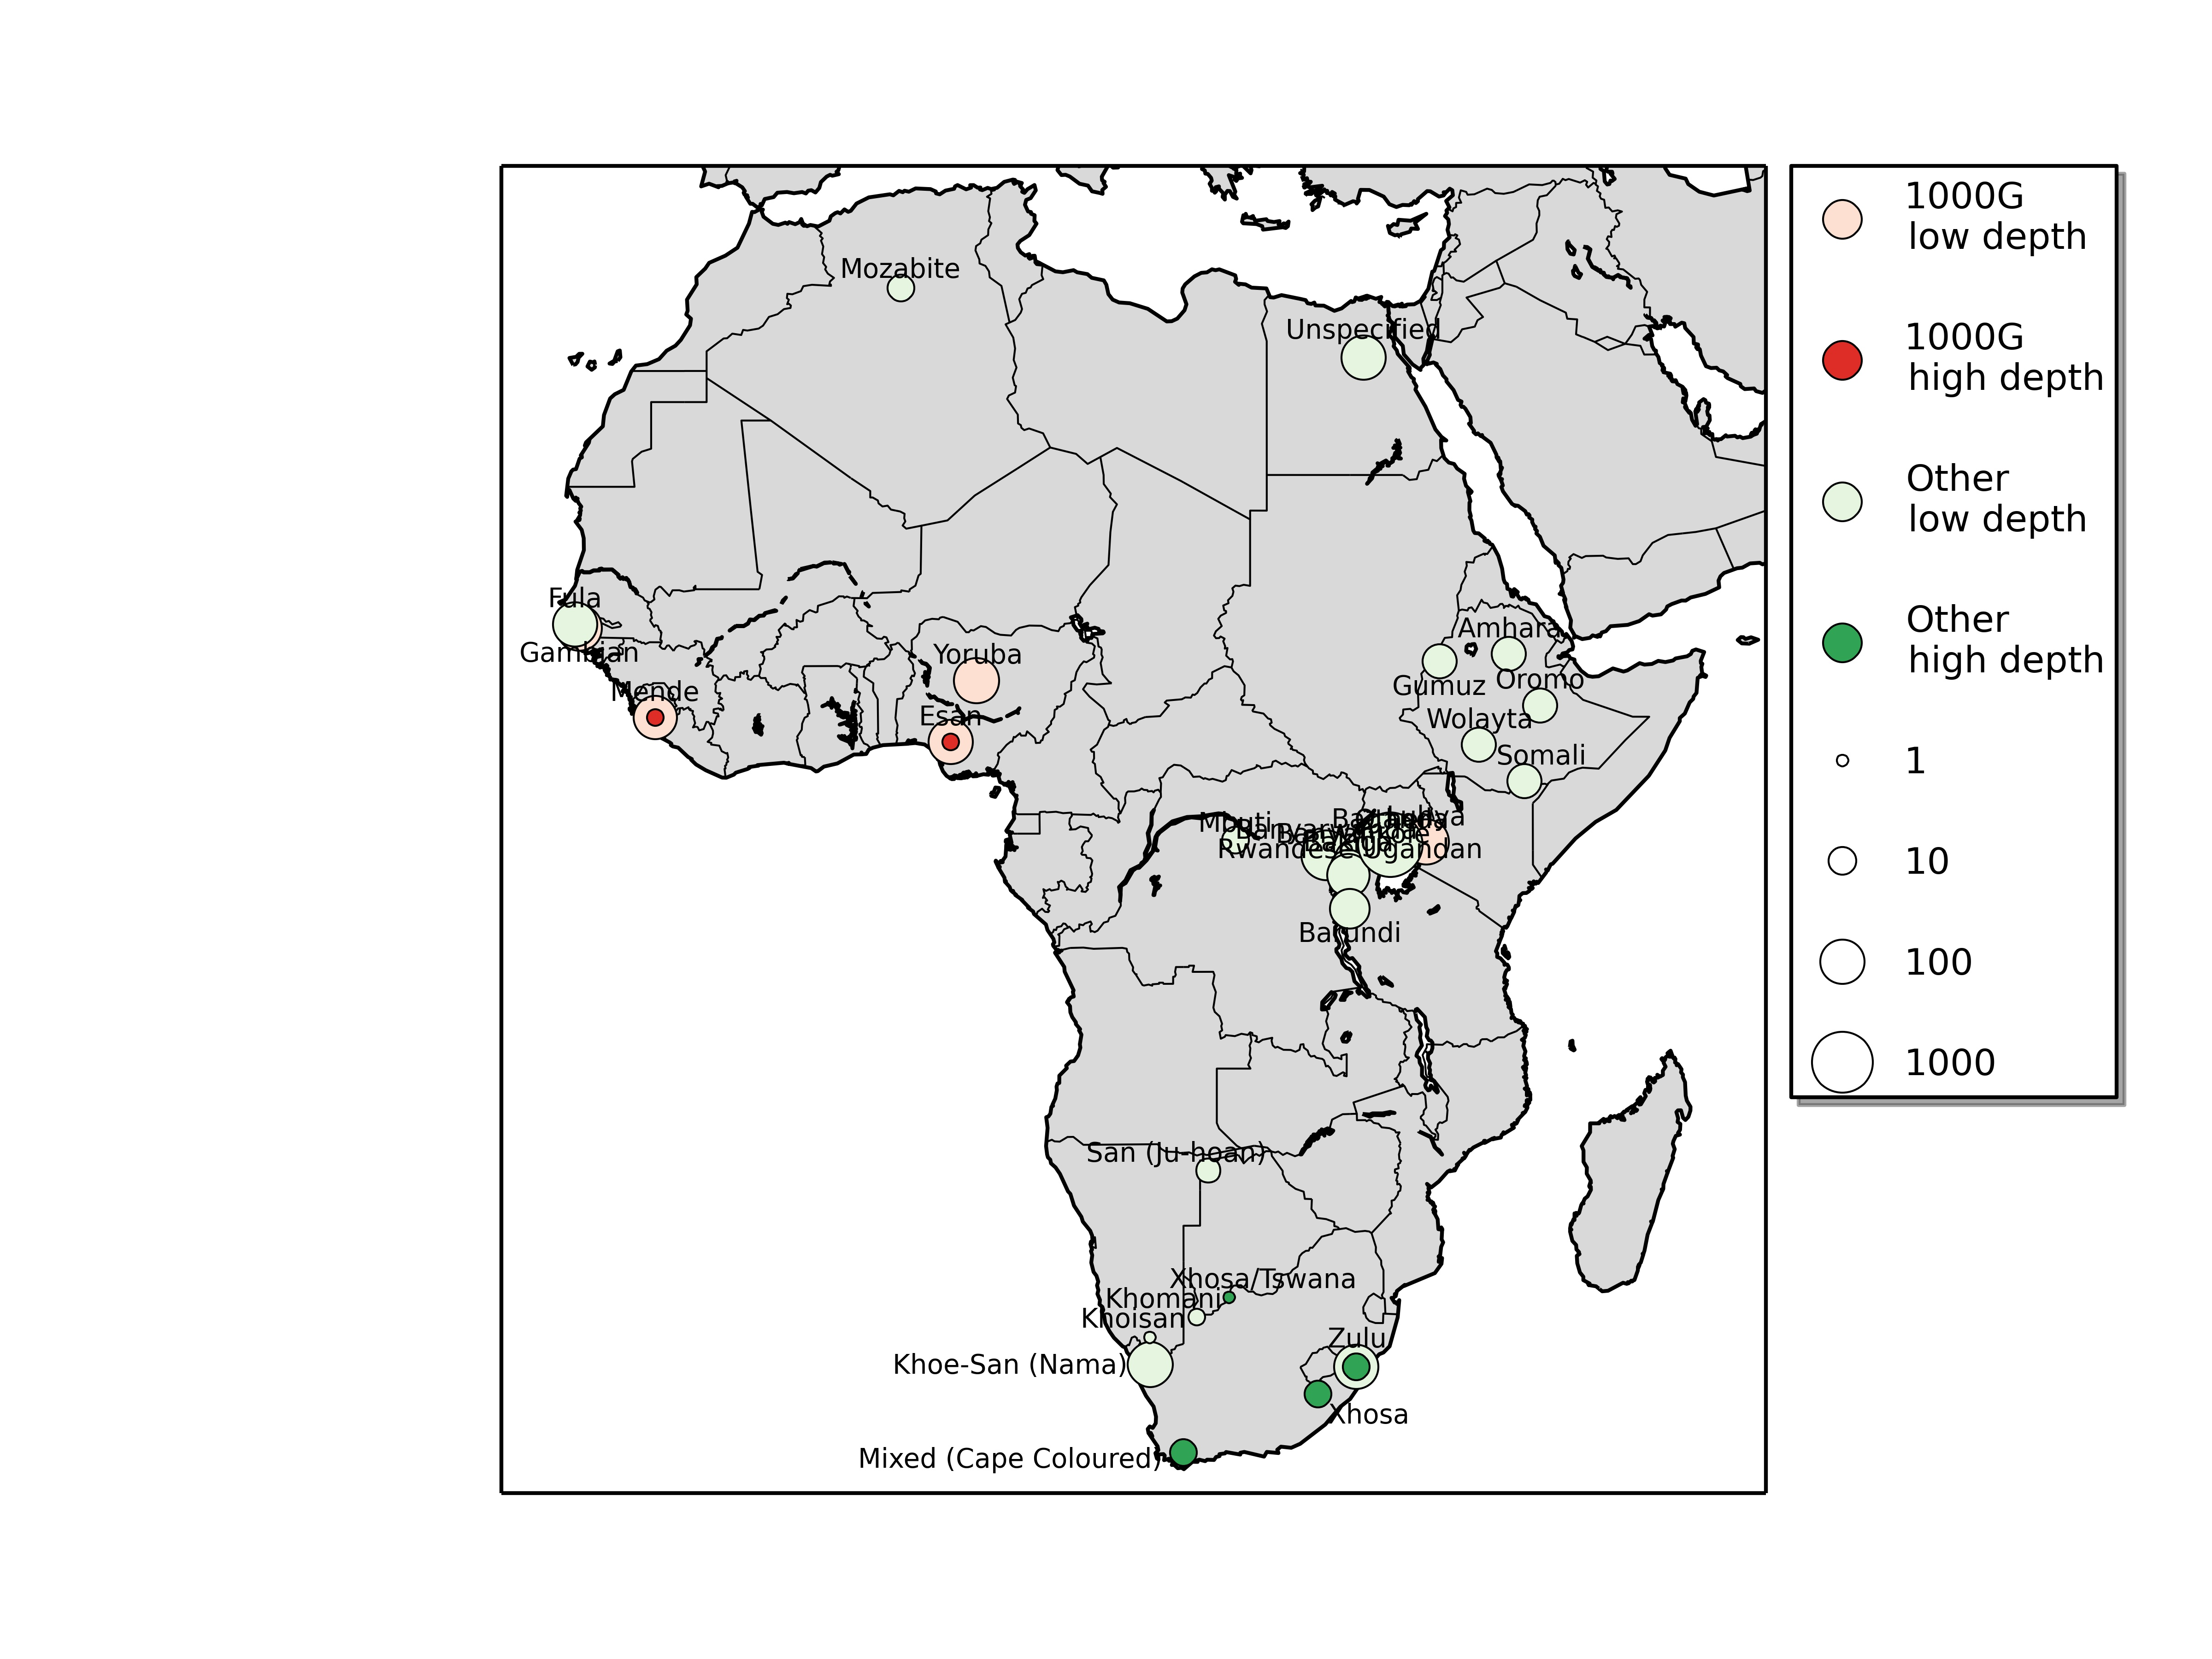
\includegraphics[width=1.0\linewidth]{tommy_2015jan21_merc_Africa_fillcontinents}
  \caption{African continent.}
\end{subfigure}%
\begin{subfigure}{.5\textwidth}
  \centering
  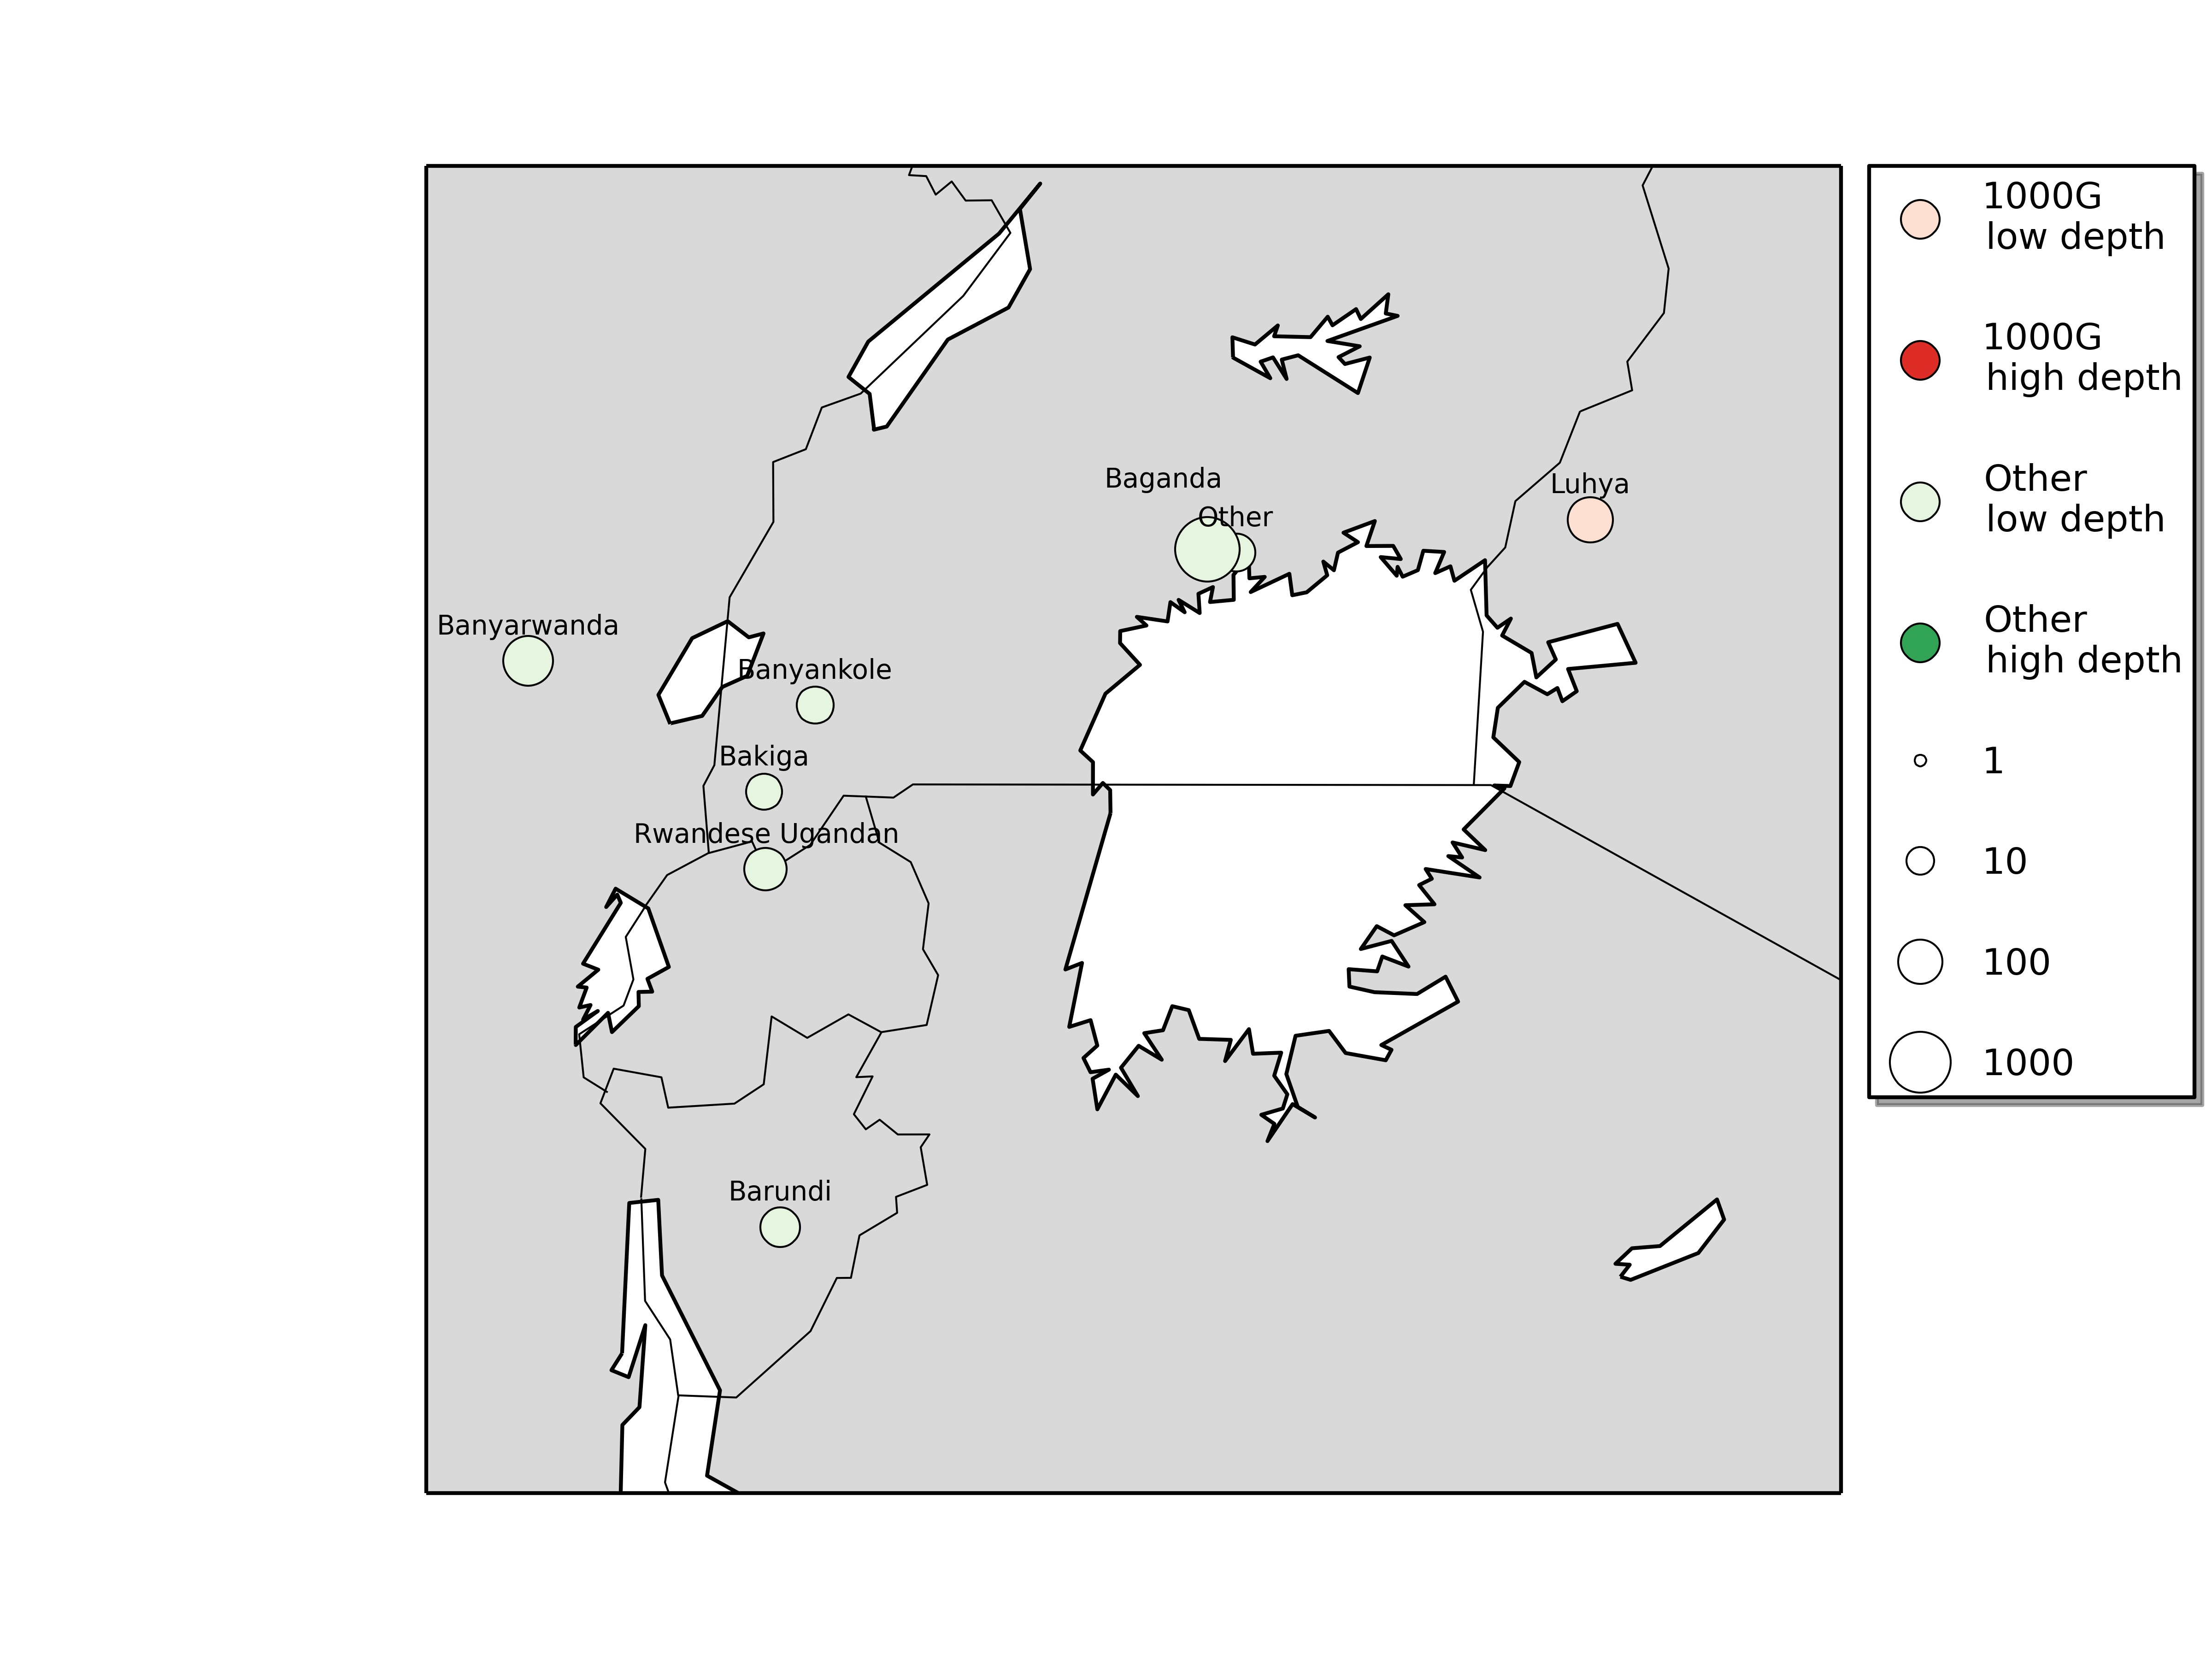
\includegraphics[width=1.0\linewidth]{tommy_2015jan21_merc_Uganda_fillcontinents}
  \caption{Southern Uganda south of the tripoint between Northern, Western and Eastern Africa.}
\end{subfigure}%
\caption{Maps showing sample location, sample count and sequencing depth of data to be included.}
\end{figure}

% I need to figure out how to avoid this table from exceeding the page width.
\begin{landscape}
\begin{longtable}{lllllll}
%\centering
\caption{Sample sets to be included in design of the African chip array}
\label{table:samples}
%\resizebox{\textwidth}{!}{%
%\begin{tabular}
\hline
Country & Ethnolinguistic group & No. & Seq depth & Source & Location & Size (TB) \\
\hline
\endhead % all the lines above this will be repeated on every page
Uganda & Baganda & 1567 & 4x & UG2G & WTSI & 40.4 \\
Uganda & Banyarwanda & 199 & 4x & UG2G & WTSI & 5.1 \\
Uganda & Rwandese Ugandan & 76 & 4x & UG2G & WTSI & 1.9 \\
Uganda & Barundi & 51 & 4x & UG2G & WTSI & 1.4 \\
Uganda & Banyankole & 36 & 4x & UG2G & WTSI & 0.93 \\
Uganda & Bakiga & 30 & 4x & UG2G & WTSI & 0.76 \\
Uganda & Other & 41 & 4x & UG2G & WTSI & 1.1 \\
Uganda & Baganda & 100 & 4x & AGVP & WTSI & 2.7 \\
South Africa & Zulu & 100 & 4x & AGVP & WTSI & 2.3 \\
Ethiopia & Amhara & 24 & 8x & AGVP & WTSI & 1.0 \\
Ethiopia & Gumuz & 24 & 8x & AGVP & WTSI & 1.0 \\
Ethiopia & Oromo & 24 & 8x & AGVP & WTSI & 1.0 \\
Ethiopia & Somali & 24 & 8x & AGVP & WTSI & 1.0 \\
Ethiopia & Wolayta & 24 & 8x & AGVP & WTSI & 1.0 \\
Egypt & Unspecified & 100 & 8x & GDAP & WTSI & 5.0 \\
South Africa & Khoe-San (Nama) & 104 & 4x & GDAP & WTSI & 3.6 \\
%Uganda & Baganda & 3 & 30x & GDAP & WTSI \\
%South Africa & Zulu & 2 & 30x & GDAP & WTSI \\
%South Africa & Khoe-San (Nama) & 3 & 30x & GDAP & WTSI \\
%Chad & Northern and Southern & 100 & 30x & GDAP & WTSI \\
%Kenya & Kalenjin & 100 & 30x & GDAP & WTSI \\
%Nigeria & Igbo & 100 & 30x & GDAP & WTSI \\
%Ghana & Ashanti & 100 & 30x & GDAP & WTSI \\
%Morocco & Moroccans & 100 & 30x & GDAP & WTSI \\
%Burkina Faso & Gouin, Kaboro, Turka & 100 & 30x & GDAP & WTSI \\
Gambia & Fula & 100 & 8x & MalariaGEN & ENA \\
Nigeria & Esan & 99 & 4x & 1000G & 1000G \\
Gambia & Gambian, Western div & 113 & 4x & 1000G & 1000G \\
Kenya & Luhya in Webuye & 116 & 4x & 1000G & 1000G \\
Sierra Leone & Mende & 85 & 4x & 1000G & 1000G \\
Nigeria & Yoruba in Ibadan & 116 & 4x & 1000G & 1000G \\
Gambia & Gambian & 2 & 30x & 1000G & Simons Foundation \\
Nigeria & Esan & 2 & 30x & 1000G & Simons Foundation \\
Sierra Leone & Mende & 2 & 30x & 1000G & Simons Foundation \\
Kenya & Luhya & 2 & 30x & Coriell & Simons Foundation \\
Kenya & Masai & 2 & 30x & Coriell & Simons Foundation \\
Kenya & Luo & 2 & 30x & Geoge Ayodo & Simons Foundation \\
Kenya & Somali & 1 & 30x & Geoge Ayodo & Simons Foundation \\
Algeria & Mozabite & 8 & 8x & HGDP/Martin et al 2014 & NCBI-SRA \\
DRC & Mbuti & 8 & 7x & HGDP/Martin et al 2014 & NCBI-SRA \\
Namibia & San (Ju-hoan) & 6 & 10x & HGDP/Martin et al 2014 & NCBI-SRA \\
Algeria & Mozabite & 2 & 30x & HGDP/Reich+Tyler-Smith & Simons Foundation and WTSI \\
%South Africa & Bantu (Tswana, Herero, Pedi, Sotho, Ovambo, Zulu) & 8 & 30x & HGDP/Reich+Tyler-Smith & Simons Foundation and WTSI \\
South Africa & \begin{tabular}[b]{@{}l@{}}Bantu\\(Tswana, Herero, Pedi, Sotho, Ovambo, Zulu)\end{tabular} & 8 & 30x & HGDP/Reich+Tyler-Smith & Simons Foundation and WTSI \\
Kenya & Bantu & 11 & 30x & HGDP/Reich+Tyler-Smith & Simons Foundation and WTSI \\
CAR & Biaka Pygmy & 23 & 30x & HGDP/Reich+Tyler-Smith & Simons Foundation and WTSI \\
Senegal & Mandenka & 22 & 30x & HGDP/Reich+Tyler-Smith & Simons Foundation and WTSI \\
DRC & Mbuti Pygmy & 12 & 30x & HGDP/Reich+Tyler-Smith & Simons Foundation and WTSI \\
Namibia & San (Ju-hoan) & 6 & 30x & HGDP/Reich+Tyler-Smith & Simons Foundation and WTSI \\
Nigeria & Yoruba & 21 & 30x & HGDP/Reich+Tyler-Smith & Simons Foundation and WTSI \\
South Africa & Khomani & 2 & 4x/9x & Kidd et al 2014 & NCBI-SRA \\
South Africa & Khomani & 2 & 30x & Brenna Henn & Simons Foundation \\
Sudan & Dinka & 3 & 30x & Michael Hammer & Simons Foundation \\
Namibia & Khoisan & 1 & 10x & Schuster et al 2009 & NCBI-SRA \\
South Africa & Xhosa/Tswana & 1 & 30x & Schuster et al 2009 & NCBI-SRA \\
North Africa & Arab-/Berber-speaking groups & ?? & 20x & Private (David Comas) &  \\
Morocco & Saharawi & 2 & 30x & David Comas & Simons Foundation \\
South Africa & Mixed (Cape Coloured) & 8 & 30x & SAHGP &  \\
South Africa & Sotho & 8 & 30x & SAHGP &  \\
South Africa & Xhosa & 8 & 30x & SAHGP &  \\
Total* &  & 3936 &  &  & 
%\end{tabular}
}
\end{longtable}
\end{landscape}